% unit: u27
% sources: sources/002-exam-2-review.txt, sources/021-exam-2-review.txt, sources/100-mit18-06scf11-ses2-12sum-pdf-download-file.txt, sources/003-exam-2-problem-solving.txt
\section{Exam 2 review}\label{sec:u27}

Part II is the heart of the course. It started from orthogonality and least squares, built
the determinant, and arrived at eigenvalues and powers of a matrix. This section gathers the
facts to have at your fingertips for the second exam, lists the quick checks that catch most
errors, and then works through review problems of the kind the exam asks, most of them from
old 18.06 exams. The exam itself covers Sections~\ref{sec:u16}--\ref{sec:u24}; differential
equations and Markov matrices (Sections~\ref{sec:u25}--\ref{sec:u26}) build on the same
ideas and are tested later.

\subsection{What to know}

\paragraph{Orthogonality and projections (Sections~\ref{sec:u16}--\ref{sec:u18}).}
The row space is orthogonal to the nullspace, and the column space is orthogonal to the left
nullspace.
Projecting $\vb{b}$ onto the line through $\vb{a}$ gives
$\vb{p}=\dfrac{\vb{a}\T\vb{b}}{\vb{a}\T\vb{a}}\,\vb{a}$ and $P=\dfrac{\vb{a}\vb{a}\T}{\vb{a}\T\vb{a}}$.
Projecting onto the column space of $A$ (independent columns): solve the normal equations
$A\T A\hat{\vb{x}}=A\T\vb{b}$, then $\vb{p}=A\hat{\vb{x}}$ and
$P=A(A\T A)^{-1}A\T$, with $P^{2}=P=P\T$. The error $\vb{e}=\vb{b}-\vb{p}$ is perpendicular
to every column of $A$. Least squares chooses $\hat{\vb{x}}$ to minimize
$\|A\vb{x}-\vb{b}\|^{2}$, and the answer is exactly this projection.

\paragraph{Orthonormal columns and Gram--Schmidt (Section~\ref{sec:u19}).}
$Q$ has orthonormal columns exactly when $Q\T Q=I$; then the projection onto its column space
is $QQ\T$, and a square $Q$ has $Q^{-1}=Q\T$. Gram--Schmidt subtracts from each new vector its
projections onto the earlier \emph{orthogonal} directions, then normalizes; the result is
$A=QR$ with $R$ upper triangular.

\paragraph{Determinants (Sections~\ref{sec:u20}--\ref{sec:u22}).}
Three properties define $\det$: $\det I=1$; exchanging rows reverses the sign; $\det$ is
linear in each row separately. Consequences: equal rows or a zero row give $0$; subtracting a
multiple of one row from another changes nothing; triangular matrices give the product of the
diagonal; $\det A=0$ exactly when $A$ is singular; $\det AB=\det A\det B$; $\det A\T=\det A$.
The big formula has $n!$ signed terms, one entry from each row and column. The cofactor
expansion is $\det A=\sum_j a_{ij}C_{ij}$, and it leads to $A^{-1}=C\T/\det A$, Cramer's rule
and $|\det A|=$ volume.

\paragraph{Eigenvalues (Sections~\ref{sec:u23}--\ref{sec:u24}).}
Solve $\det(A-\lambda I)=0$, then find $\Nul{A-\lambda I}$. The sum of the eigenvalues is the
trace, the product is the determinant. With $n$ independent eigenvectors,
$A=X\Lambda X^{-1}$, $A^{k}=X\Lambda^{k}X^{-1}$, and
$\vb{u}_k=A^{k}\vb{u}_0=\sum c_i\lambda_i^{k}\vb{x}_i$ where $X\vb{c}=\vb{u}_0$. Distinct
eigenvalues guarantee independent eigenvectors; a repeated eigenvalue may not.

\subsection{Quick checks}

An exam rewards answers that are checked as they are produced. The cheapest checks:
\begin{itemize}
  \item eigenvalues: their sum must equal the trace and their product the determinant, and
  $A\vb{x}=\lambda\vb{x}$ can be verified in seconds;
  \item projections: $P^{2}=P$, $P\T=P$, $P\vb{a}=\vb{a}$ for vectors already in the
  subspace, and the error must be perpendicular to the subspace;
  \item Gram--Schmidt: each new vector must have zero dot product with the earlier ones;
  \item inverses and factorizations: substitute $k=1$ into a formula for $A^{k}$, multiply
  $A\,C\T$ to see $(\det A)I$, and expand a determinant along a second row or column.
\end{itemize}

\subsection{Solved review problems}

\begin{example}[Projection onto a line, and its powers]\label{ex:u27-projection}
Let $\vb{a}=(2,1,2)$. (a) Find the projection matrix $P$ onto the line through $\vb{a}$.
(b) Find its rank, column space and eigenvalues, and an eigenvector for each eigenvalue.
(c) Solve $\vb{u}_{k+1}=P\vb{u}_k$ with $\vb{u}_0=(9,9,0)$.

(a) Here $\vb{a}\T\vb{a}=9$, so
\[
  P=\frac{\vb{a}\vb{a}\T}{\vb{a}\T\vb{a}}=\frac19\begin{bmatrix} 4&2&4\\ 2&1&2\\ 4&2&4\end{bmatrix}.
\]

(b) Every column is a multiple of $\vb{a}$, so $\rank P=1$ and $\Col{P}$ is the line through
$\vb{a}$. A rank-one $3\times3$ matrix has a two-dimensional nullspace, so $\lambda=0$ is an
eigenvalue twice, with eigenvectors such as $(1,-2,0)$ and $(1,0,-1)$, the vectors
perpendicular to $\vb{a}$. The trace $\tfrac{4+1+4}{9}=1$ gives the third eigenvalue
$\lambda=1$, with eigenvector $\vb{a}$ itself: $P\vb{a}=\vb{a}(\vb{a}\T\vb{a})/9=\vb{a}$.

(c) The first step projects $\vb{u}_0$ onto the line:
\[
  \vb{u}_1=P\vb{u}_0=\frac{\vb{a}\T\vb{u}_0}{\vb{a}\T\vb{a}}\,\vb{a}=\frac{18+9+0}{9}\,\vb{a}=3\vb{a}=(6,3,6).
\]
Since $\vb{u}_1$ is already on the line, projecting again changes nothing: $P^{2}=P$, so
$\vb{u}_k=P^{k}\vb{u}_0=P\vb{u}_0=(6,3,6)$ for every $k\ge1$. In the eigenvector language of
Section~\ref{sec:u24}, $\vb{u}_0=3\vb{a}+(3,6,-6)$, where $(3,6,-6)$ is perpendicular to
$\vb{a}$ and has $\lambda=0$; that part disappears after one step and the $\lambda=1$ part
$3\vb{a}$ stays forever. For a matrix that is not a projection one would find all eigenvalues
and eigenvectors and use $\vb{u}_k=\sum c_i\lambda_i^{k}\vb{x}_i$.
\end{example}

\begin{example}[Best line through the origin]\label{ex:u27-leastsq}
Fit the line $y=Dt$ to the data points $(t,y)=(1,4)$, $(2,5)$, $(3,8)$, and say what vector
is projected onto what line.

The three equations $1\cdot D=4$, $2\cdot D=5$, $3\cdot D=8$ form $A\vb{x}=\vb{b}$ with a
single column $A=(1,2,3)$ and $\vb{b}=(4,5,8)$; they have no solution. The normal equation is
\[
  A\T A\,\hat D=A\T\vb{b}:\qquad 14\,\hat D=4+10+24=38,\qquad \hat D=\frac{19}{7}\approx2.71 .
\]
There are two pictures (Figure~\ref{fig:u27-fit}). In the $ty$-plane we fit a line to three
points; the errors are the vertical distances. In $\R^{3}$ we project the vector
$\vb{b}=(4,5,8)$ onto the line through $(1,2,3)$, the column space of $A$:
$\vb{p}=\tfrac{19}{7}(1,2,3)=\tfrac17(19,38,57)$ and
$\vb{e}=\vb{b}-\vb{p}=\tfrac17(9,-3,-1)$. Check: $\vb{e}\cdot(1,2,3)=\tfrac17(9-6-3)=0$.
The components of $\vb{e}$ are exactly the vertical errors in the first picture.
\end{example}

\begin{figure}[ht]\centering
\begin{tikzpicture}
\begin{axis}[width=0.55\textwidth,height=0.42\textwidth,xmin=0,xmax=4,ymin=0,ymax=9.5,
  axis lines=left,xlabel={$t$},ylabel={$y$},xtick={1,2,3},ytick={2,4,6,8},clip=false]
  \addplot[blue,thick,domain=0:3.4] {19/7*x} node[pos=0.55,above left] {$y=\tfrac{19}{7}t$};
  \addplot[red,dashed] coordinates {(1,4) (1,19/7)};
  \addplot[red,dashed] coordinates {(2,5) (2,38/7)};
  \addplot[red,dashed] coordinates {(3,8) (3,57/7)};
  \addplot[only marks,mark=*,mark size=2pt] coordinates {(1,4) (2,5) (3,8)};
  \node[left,red,font=\small] at (axis cs:1,3.35) {$e_1=\tfrac97$};
  \node[below right,red,font=\small] at (axis cs:2,5) {$e_2=-\tfrac37$};
  \node[below right,red,font=\small] at (axis cs:3,8) {$e_3=-\tfrac17$};
\end{axis}
\end{tikzpicture}
\caption{The least-squares line through the origin for Example~\ref{ex:u27-leastsq}. The
vertical errors $e_i=y_i-\tfrac{19}{7}t_i$ are the components of the error vector
$\vb{e}=\vb{b}-\vb{p}$, which is perpendicular to the column $(1,2,3)$ in $\R^{3}$.}
\label{fig:u27-fit}
\end{figure}

\begin{example}[Gram--Schmidt in a plane]\label{ex:u27-gs}
The vectors $\vb{a}_1=(1,2,3)$ and $\vb{a}_2=(1,1,1)$ span a plane. Find two orthogonal
vectors in it, then an orthonormal pair.

Keep $\vb{a}_1$. From $\vb{a}_2$ subtract its projection onto $\vb{a}_1$:
\[
  \vb{B}=\vb{a}_2-\frac{\vb{a}_1\T\vb{a}_2}{\vb{a}_1\T\vb{a}_1}\,\vb{a}_1
  =\begin{bmatrix} 1\\ 1\\ 1\end{bmatrix}-\frac{6}{14}\begin{bmatrix} 1\\ 2\\ 3\end{bmatrix}
  =\begin{bmatrix} 1-\tfrac37\\ 1-\tfrac67\\ 1-\tfrac97\end{bmatrix}
  =\frac17\begin{bmatrix} 4\\ 1\\ -2\end{bmatrix}.
\]
Check: $\vb{a}_1\cdot(4,1,-2)=4+2-6=0$. Dividing by the lengths $\sqrt{14}$ and
$\sqrt{16+1+4}=\sqrt{21}$ gives the orthonormal pair
$\vb{q}_1=(1,2,3)/\sqrt{14}$, $\vb{q}_2=(4,1,-2)/\sqrt{21}$. The square roots appear only in
this last step, so it pays to postpone it.
\end{example}

\begin{example}[What the eigenvalues alone tell]\label{ex:u27-eigfacts}
A $4\times4$ matrix $A$ has eigenvalues $\lambda_1,\lambda_2,\lambda_3,\lambda_4$. When is it
invertible? What are $\det A^{-1}$ and $\tr(A+I)$?

$A$ is invertible exactly when no $\lambda_i$ is $0$: an eigenvalue $0$ means a nonzero vector
in the nullspace, and $\det A=\lambda_1\lambda_2\lambda_3\lambda_4$. The eigenvalues of
$A^{-1}$ are $1/\lambda_i$ (Section~\ref{sec:u23}), so
$\det A^{-1}=\dfrac{1}{\lambda_1\lambda_2\lambda_3\lambda_4}$. Adding $I$ adds $1$ to every
eigenvalue (Section~\ref{sec:u23}), so
$\tr(A+I)=\lambda_1+\lambda_2+\lambda_3+\lambda_4+4$, which is also $\tr A+4$ directly.
\end{example}

\begin{example}[Tridiagonal determinants repeat with period six]\label{ex:u27-tridiag}
Let $A_n$ be the $n\times n$ tridiagonal matrix with $1$'s on the diagonal and on both
neighbouring diagonals, and $D_n=\det A_n$. Find a recurrence for $D_n$ and solve it.

\emph{Recurrence.} Expand along the first row, which has $1$'s in columns~1 and~2 only. The
$(1,1)$ cofactor is $D_{n-1}$. The $(1,2)$ cofactor is $-1$ times the determinant of $A_n$
without row~1 and column~2; that matrix has first column $(1,0,\dots,0)$, and expanding
down it leaves $A_{n-2}$. So
\[
  D_n=D_{n-1}-D_{n-2},\qquad D_1=1,\quad D_2=\begin{vmatrix} 1&1\\ 1&1\end{vmatrix}=0 .
\]
\emph{As a matrix system.} With $\vb{u}_n=(D_n,D_{n-1})$,
$\vb{u}_n=\left[\begin{smallmatrix} 1&-1\\ 1&0\end{smallmatrix}\right]\vb{u}_{n-1}$. The
characteristic equation is $\lambda^{2}-\lambda+1=0$, so
\[
  \lambda=\frac{1\pm\sqrt{1-4}}{2}=\frac12\pm\frac{\sqrt3}{2}\,i=e^{\pm i\pi/3}.
\]
Both have $|\lambda|^{2}=\tfrac14+\tfrac34=1$: the sequence neither grows nor decays. Since
$\lambda^{6}=e^{\pm2\pi i}=1$, the matrix $M=\left[\begin{smallmatrix} 1&-1\\ 1&0\end{smallmatrix}\right]$
is diagonalizable with $\Lambda^{6}=I$, so $M^{6}=X\Lambda^{6}X^{-1}=I$ and the sequence
repeats every six steps. Running the recurrence:
\[
  D_1,\dots,D_6=1,\;0,\;-1,\;-1,\;0,\;1,\qquad\text{then } D_7=1,\ D_8=0,\dots
\]
so $D_n$ depends only on $n$ modulo $6$.
\end{example}

\begin{example}[A family of symmetric matrices]\label{ex:u27-family}
Let $A_n$ be symmetric with zeros on the diagonal and $1,2,\dots,n-1$ just above and below
it, for instance
\[
  A_3=\begin{bmatrix} 0&1&0\\ 1&0&2\\ 0&2&0\end{bmatrix},\qquad
  A_4=\begin{bmatrix} 0&1&0&0\\ 1&0&2&0\\ 0&2&0&3\\ 0&0&3&0\end{bmatrix}.
\]
(a) Find the projection matrix onto $\Col{A_3}$. (b) Find the eigenvalues and eigenvectors of
$A_3$. (c) Find the projection onto $\Col{A_4}$. (d) Show that $A_n$ is singular for odd $n$ and
invertible for even $n$.

(a) Column~3 is twice column~1, so $\Col{A_3}$ is the plane spanned by $(0,1,0)$ and
$(1,0,2)$. These two columns are already orthogonal, so $P$ is the sum of the two
projections onto lines:
\[
  P=\begin{bmatrix} 0\\ 1\\ 0\end{bmatrix}\begin{bmatrix} 0&1&0\end{bmatrix}
   +\frac15\begin{bmatrix} 1\\ 0\\ 2\end{bmatrix}\begin{bmatrix} 1&0&2\end{bmatrix}
  =\begin{bmatrix} \tfrac15&0&\tfrac25\\ 0&1&0\\ \tfrac25&0&\tfrac45\end{bmatrix}.
\]
The formula $A(A\T A)^{-1}A\T$ with these two columns gives the same matrix. Check: $P$
fixes all three columns of $A_3$.

(b) $\det(A_3-\lambda I)=-\lambda^{3}+5\lambda=-\lambda(\lambda^{2}-5)$, so
$\lambda=0,\sqrt5,-\sqrt5$ (trace check: the sum is $0$). The eigenvectors are
$(-2,0,1)$ for $0$ and $(1,\pm\sqrt5,2)$ for $\pm\sqrt5$; for instance
$A_3(1,\sqrt5,2)=(\sqrt5,\,5,\,2\sqrt5)=\sqrt5\,(1,\sqrt5,2)$. The eigenvector
$(-2,0,1)$ spans the nullspace, perpendicular to $\Col{A_3}$, so $P=I-\tfrac15(-2,0,1)(-2,0,1)\T$
is another route to (a).

(c) If $A_4$ is invertible, its column space is all of $\R^{4}$ and the projection is
$P=I$. Expanding along row~1 (only the entry $1$ in column~2), then down the first column of
the resulting $3\times3$ minor,
\[
  \det A_4=-1\cdot\begin{vmatrix} 1&2&0\\ 0&0&3\\ 0&3&0\end{vmatrix}
  =-1\cdot1\cdot\begin{vmatrix} 0&3\\ 3&0\end{vmatrix}=-1\cdot(-9)=9\neq0 .
\]
So $P=I$.

(d) Expand $D_n=\det A_n$ along the last row, whose only nonzero entry is $n-1$ in column
$n-1$. Its minor has last column $(0,\dots,0,n-1)$; expanding down that column leaves
$A_{n-2}$. With the sign $(-1)^{n+(n-1)}=-1$,
\[
  D_n=-(n-1)^{2}\,D_{n-2},\qquad D_1=0,\quad D_2=-1 .
\]
So $D_n=0$ for every odd $n$, and for even $n$ the determinant is
$\pm\bigl(1\cdot3\cdot5\cdots(n-1)\bigr)^{2}\neq0$: for example $D_4=-9D_2=9$ and
$D_6=-25D_4=-225$.
\end{example}

\begin{example}[The big formula when many entries are zero]\label{ex:u27-bigformula}
For the matrix below, find $\det A$ from the big formula, the cofactors
$C_{11},\dots,C_{14}$, and the first column of $A^{-1}$:
\[
  A=\begin{bmatrix} 1&2&3&4\\ 5&6&7&8\\ 0&0&9&10\\ 0&0&11&12\end{bmatrix}.
\]

\emph{Big formula.} Of the $24$ terms, only those avoiding the four zeros survive. Rows~3
and~4 must use columns~3 and~4, so rows~1 and~2 use columns~1 and~2: four terms in all. A
term's sign is that of its column permutation:
\[
  \det A=+1\cdot6\cdot9\cdot12-1\cdot6\cdot10\cdot11-2\cdot5\cdot9\cdot12+2\cdot5\cdot10\cdot11
  =648-660-1080+1100=8 .
\]
(The permutations are $(1,2,3,4)$, $(1,2,4,3)$, $(2,1,3,4)$ and $(2,1,4,3)$, with $0$, $1$, $1$
and $2$ exchanges.)

\emph{Cofactors.} $C_{11}=\det\left[\begin{smallmatrix} 6&7&8\\ 0&9&10\\ 0&11&12\end{smallmatrix}\right]=6(108-110)=-12$
and $C_{12}=-\det\left[\begin{smallmatrix} 5&7&8\\ 0&9&10\\ 0&11&12\end{smallmatrix}\right]=-5(-2)=10$,
each expanded down its first column. $C_{13}=C_{14}=0$ without computation: their minors have
first two columns $(5,0,0)$ and $(6,0,0)$, which are dependent. Check:
$\det A=1\cdot(-12)+2\cdot10+0+0=8$.

\emph{First column of $A^{-1}$.} By the formula $A^{-1}=C\T/\det A$ of Section~\ref{sec:u22} it is the first row of
cofactors divided by the determinant:
\[
  \frac{1}{\det A}\,(C_{11},C_{12},C_{13},C_{14})=\frac18\,(-12,10,0,0)=\Bigl(-\frac32,\frac54,0,0\Bigr).
\]
A third check: $A$ is block triangular, and
$\det\left[\begin{smallmatrix} 1&2\\ 5&6\end{smallmatrix}\right]\det\left[\begin{smallmatrix} 9&10\\ 11&12\end{smallmatrix}\right]=(-4)(-2)=8$.
\end{example}

\subsection{Exercises}

\begin{exercise}\label{exr:u27-line}
Fit the best straight line $y=C+Dt$ to the points $(-1,1)$, $(0,2)$, $(1,4)$, and find the
error vector.
\end{exercise}
\begin{solution}
$A=\left[\begin{smallmatrix} 1&-1\\ 1&0\\ 1&1\end{smallmatrix}\right]$, $\vb{b}=(1,2,4)$.
Because the times add to zero, the columns of $A$ are orthogonal and
$A\T A=\left[\begin{smallmatrix} 3&0\\ 0&2\end{smallmatrix}\right]$, while $A\T\vb{b}=(7,3)$.
So $\hat C=\tfrac73$, $\hat D=\tfrac32$. The fitted values are
$\tfrac73+\tfrac32t=\tfrac56,\tfrac73,\tfrac{23}{6}$ at $t=-1,0,1$, and
$\vb{e}=(1,2,4)-(\tfrac56,\tfrac{14}{6},\tfrac{23}{6})=(\tfrac16,-\tfrac13,\tfrac16)$, which is
perpendicular to both columns: $\tfrac16-\tfrac13+\tfrac16=0$ and $-\tfrac16+0+\tfrac16=0$.
\end{solution}

\begin{exercise}\label{exr:u27-eigalg}
A $3\times3$ matrix $A$ has eigenvalues $1,2,3$. Find $\det A$, $\tr A$, the eigenvalues of
$A^{2}-A$, and $\det(A^{2}-A)$. Is $A$ diagonalizable?
\end{exercise}
\begin{solution}
$\det A=1\cdot2\cdot3=6$ and $\tr A=6$. By Section~\ref{sec:u23} the
eigenvalues of $A^{2}-A$ are $\lambda^{2}-\lambda=0,2,6$, so $\det(A^{2}-A)=0$: the matrix
$A^{2}-A=A(A-I)$ is singular, as it must be since $A-I$ has the eigenvalue $0$. $A$ is
diagonalizable because its three eigenvalues are distinct (Section~\ref{sec:u24}).
\end{solution}

\begin{exercise}\label{exr:u27-tridiag2}
Let $T_n$ be tridiagonal with $2$'s on the diagonal and $-1$'s on the two neighbouring
diagonals. Use cofactors to show $\det T_n=2\det T_{n-1}-\det T_{n-2}$, and find $\det T_n$.
\end{exercise}
\begin{solution}
Expanding along the first row exactly as in Example~\ref{ex:u27-tridiag}: the $(1,1)$ term
gives $2\det T_{n-1}$; the $(1,2)$ entry $-1$ has cofactor $-1$ times a determinant whose
first column is $(-1,0,\dots,0)$, which equals $-\det T_{n-2}$. Altogether
$\det T_n=2\det T_{n-1}+(-1)(-1)(-\det T_{n-2})=2\det T_{n-1}-\det T_{n-2}$. With
$\det T_1=2$ and $\det T_2=4-1=3$, the recurrence gives $4,5,6,\dots$; by induction
$\det T_n=n+1$, since $2n-(n-1)=n+1$. (In matrix form, $\left[\begin{smallmatrix} 2&-1\\ 1&0\end{smallmatrix}\right]$
has the repeated eigenvalue $1$ and only one eigenvector, which is why the answer grows
linearly instead of like a power.)
\end{solution}
